\documentclass[12pt, twoside]{article}
\usepackage[letterpaper, margin=1in, headsep=0.5in]{geometry}
\usepackage[english]{babel}
\usepackage[utf8]{inputenc}
\usepackage{amsmath}
\usepackage{amsfonts}
\usepackage{amssymb}
\usepackage{tikz}
\usetikzlibrary{quotes, angles}
\usepackage{graphicx}
%\usepackage{pgfplots}
%\pgfplotsset{width=10cm,compat=1.9}
%\usepgfplotslibrary{statistics}
%\usepackage{pgfplotstable}
%\usepackage{tkz-fct}
%\usepackage{venndiagram}
\usepackage{enumitem}
\usepackage{multicol}


\usepackage{fancyhdr}
\pagestyle{fancy}
\fancyhf{}
\fancyhead[LE]{\thepage}
\fancyhead[RO]{\thepage \\Name: \hspace{4cm} \,\\}
\fancyhead[LO]{BECA / Mr. Segal, Dr. Huson / Geometry\\* Unit 14: Congruence transformations \\ 13 June 2022}

\renewcommand{\headrulewidth}{0pt}

\begin{document}
\subsubsection*{14.2 Classwork: Formal constructions with compass and straight edge}
\begin{enumerate}
\item Complete the construction of an equilateral triangle with one side as $\overline{XY}$. Show all construction marks, but make no extra lines. \vspace{6cm}
\begin{center}
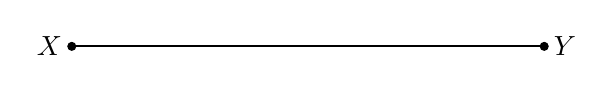
\begin{tikzpicture}
  \draw [-, thick] (0,0)--(6,0);
  \draw [fill] (0,0) circle [radius=0.05] node[left]{$X$};
  \draw [fill] (6,0) circle [radius=0.05] node[right]{$Y$};
\end{tikzpicture}
\end{center} \vspace{1cm}
\begin{enumerate}
  \item Identify two circles in the construction. For each, name the center of the circle and the radius.  \vspace{2cm}
  \item Assuming that the third vertex of the triangle is point $Z$, explain why the distance from $X$ to $Z$ is the same as the distance from $X$ to $Y$.
\end{enumerate} \vspace{2cm}

\item Using a compass and straightedge, construct a line segment $\overline{AC}$ on the ray $\overrightarrow{AB}$ that is twice the length of $\overline{AB}$.\vspace{2cm}
  \begin{center}
  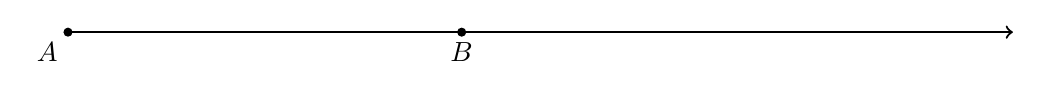
\begin{tikzpicture}
    %\draw [thick, <->] (-7.4,0) -- (10.4,0) node [right] {$x$};
    %\draw [thick, <->] (0,-6.4)--(0,10.4) node [above] {$y$};
    \draw [thick, ->]
    (0,0) node[below left] {$A$}--
    (5,0) node[below] {$B$}--
    (12,0);
    \draw [fill] (0,0) circle[radius=0.05];
    \draw [fill] (5,0) circle[radius=0.05];
  \end{tikzpicture}
\end{center}

\newpage
\item Complete the construction of a perpendicular bisector of $\overline{AB}$. Label the midpoint $M$. Show all construction marks, but make no extra lines. \vspace{2cm}
  \begin{center}
  \begin{tikzpicture}
    \draw [-, thick] (0,0)--(3,4);
    \draw [fill] (0,0) circle [radius=0.05] node[below right]{$A$};
    \draw [fill] (3,4) circle [radius=0.05] node[above right]{$B$};
  \end{tikzpicture}
  \end{center} \vspace{1cm}

\item Complete the construction of a line perpendicular to line $l$ through the point $P$. Show all construction marks, but make no extra lines. \vspace{1cm}
\begin{center}
\begin{tikzpicture}
  \draw [<->, thick] (-5,0)--(7,0)node[below]{$l$}--(8,0);
  \draw [fill] (3,3) circle [radius=0.05] node[above left]{$P$};
\end{tikzpicture}
\end{center} 
\vspace{3cm}

\newpage
\item Bisect the given angle. \vspace{2cm}
  \begin{center}
  \begin{tikzpicture}
    \draw [<->, thick] (80:6)--(0,0)--(20:6);
    \draw [fill] (0,0) circle [radius=0.05] node[below]{$A$};
  \end{tikzpicture}
  \end{center} \vspace{0.5cm}

\item Construct a perpendicular to $\overline{AB}$ though $C$.\\
%\hspace{1cm} Given the line  $l$ and point $P$.
  \vspace{2cm}
  \begin{center}
  \begin{tikzpicture}
    \draw [<->, thick] (0,0)--(11,0)--(6,3)--cycle;
    \draw [fill] (0,0) circle [radius=0.05] node[left]{$A$};
    \draw [fill] (11,0) circle [radius=0.05] node[right]{$B$};
    \draw [fill] (6,3) circle [radius=0.05] node[above right]{$C$};
  \end{tikzpicture}
  \end{center} \vspace{5cm}

\newpage
\item Using a compass and straightedge, construct $M$, the midpoint of $\overline{AB}$. Then draw the median $\overline{CM}$.
\vspace{2cm}
  \begin{center}
  \begin{tikzpicture}[scale=1.2]
    %\draw [thick, <->] (-7.4,0) -- (10.4,0) node [right] {$x$};
    %\draw [thick, <->] (0,-6.4)--(0,10.4) node [above] {$y$};

    \draw [thick]
    (5,-1) node[below left] {$A$}--
    (8,2) node[right] {$B$}--
    (1,0) node[below left] {$C$}--cycle;
  \end{tikzpicture}
\end{center} \vspace{2cm}

\item Using a compass and straightedge, dilate $\triangle ABC$ by a scale factor of 2 centered at $A$.\\[0.25cm] Construct line segment $\overline{AB'}$ that is twice the length of $\overline{AB}$ and $\overline{AC'}$ that is twice the length of $\overline{AC}$. Draw $\overline{A'B'}$ to complete the desired triangle, $\triangle AB'C'$. \vspace{2cm}
  \begin{center}
  \begin{tikzpicture}
    %\draw [thick, <->] (-7.4,0) -- (10.4,0) node [right] {$x$};
    %\draw [thick, <->] (0,-6.4)--(0,10.4) node [above] {$y$};
    \draw [thick, <->]
    (10,5)--
    (4,2) node[above left] {$C$}--
    (0,0) node[below left] {$A$}--
    (5,-1) node[below] {$B$}--
    (12,-2.4);
    \draw [thick] (4,2)--(5,-1);
    \draw [fill] (0,0) circle[radius=0.05];
    \draw [fill] (5,-1) circle[radius=0.05];
    \draw [fill] (4,2) circle[radius=0.05];
  \end{tikzpicture}
\end{center}


\end{enumerate}
\end{document}

